\documentclass[12pt]{article}

% PACKAGES
\usepackage[margin = 0.6in]{geometry}
\usepackage{amsfonts}
\usepackage{amsmath}
\usepackage{amssymb}
\usepackage{multicol}
\usepackage{graphicx}
\usepackage{float}
\usepackage{xcolor}
\usepackage{amsthm}
\usepackage{dsfont}
\usepackage{hyperref}
\usepackage{setspace}
\usepackage{algorithm}
\usepackage{algpseudocode}
\usepackage{subcaption}
% MACROS
% Set Theory
\def\N{\mathbb{N}}
\def\R{\mathbb{R}}
\def\C{\mathbb{C}}
\def\Z{\mathbb{Z}}
%\def\^{\hat}
\def\-{\vec}
\def\d{\partial}
\def\!{\boldsymbol}
\def\X{\times}
%\def\-{\bar}
\def\bf{\textbf}
\def\l{\left}
\def\r{\right}
\def\~{\tilde}
\date{August 2022}
\doublespacing
\begin{document}

\begin{titlepage}
    \begin{center}
        \vspace*{1cm}
            
        \Huge
        \textbf{Multifidelity Finite Basis Physics Informed Neural Networks}
            
            
        \vfill
            
        
        Name: Damien Beecroft\\
        Hosting Site: Pacific Northwest National Lab\\
        Mentors: Amanda Howard and Panos Stinis\\
        \vspace{2cm}
        \begin{flushleft}
       	Mentor's Signature:\\
       	\end{flushleft}
       	\Large
        
            
    \end{center}
\end{titlepage}

\section*{Abstract}
\begin{singlespace}
Physics informed neural networks (PINNs) struggle to successfully learn solutions to differential equations that exhibit high-frequency oscillations or multi-scale behavior. Multilevel finite basis physics informed neural networks (FBPINNs) tackle this problem by recursively discretizing the solution domain and training coupled neural networks on the subdomains. In this work we integrate multifidelity methods into multilevel FBPINNs to improve convergence. We tested this method on a collection of test problems and analyzed the errors and solution structure to determine the quality of the results. This project can benefit anyone that is trying to model a differential equation that classical numerical or analytical methods struggle to solve.
\end{singlespace}
\vspace{1cm}
\begin{figure}[H]
\center
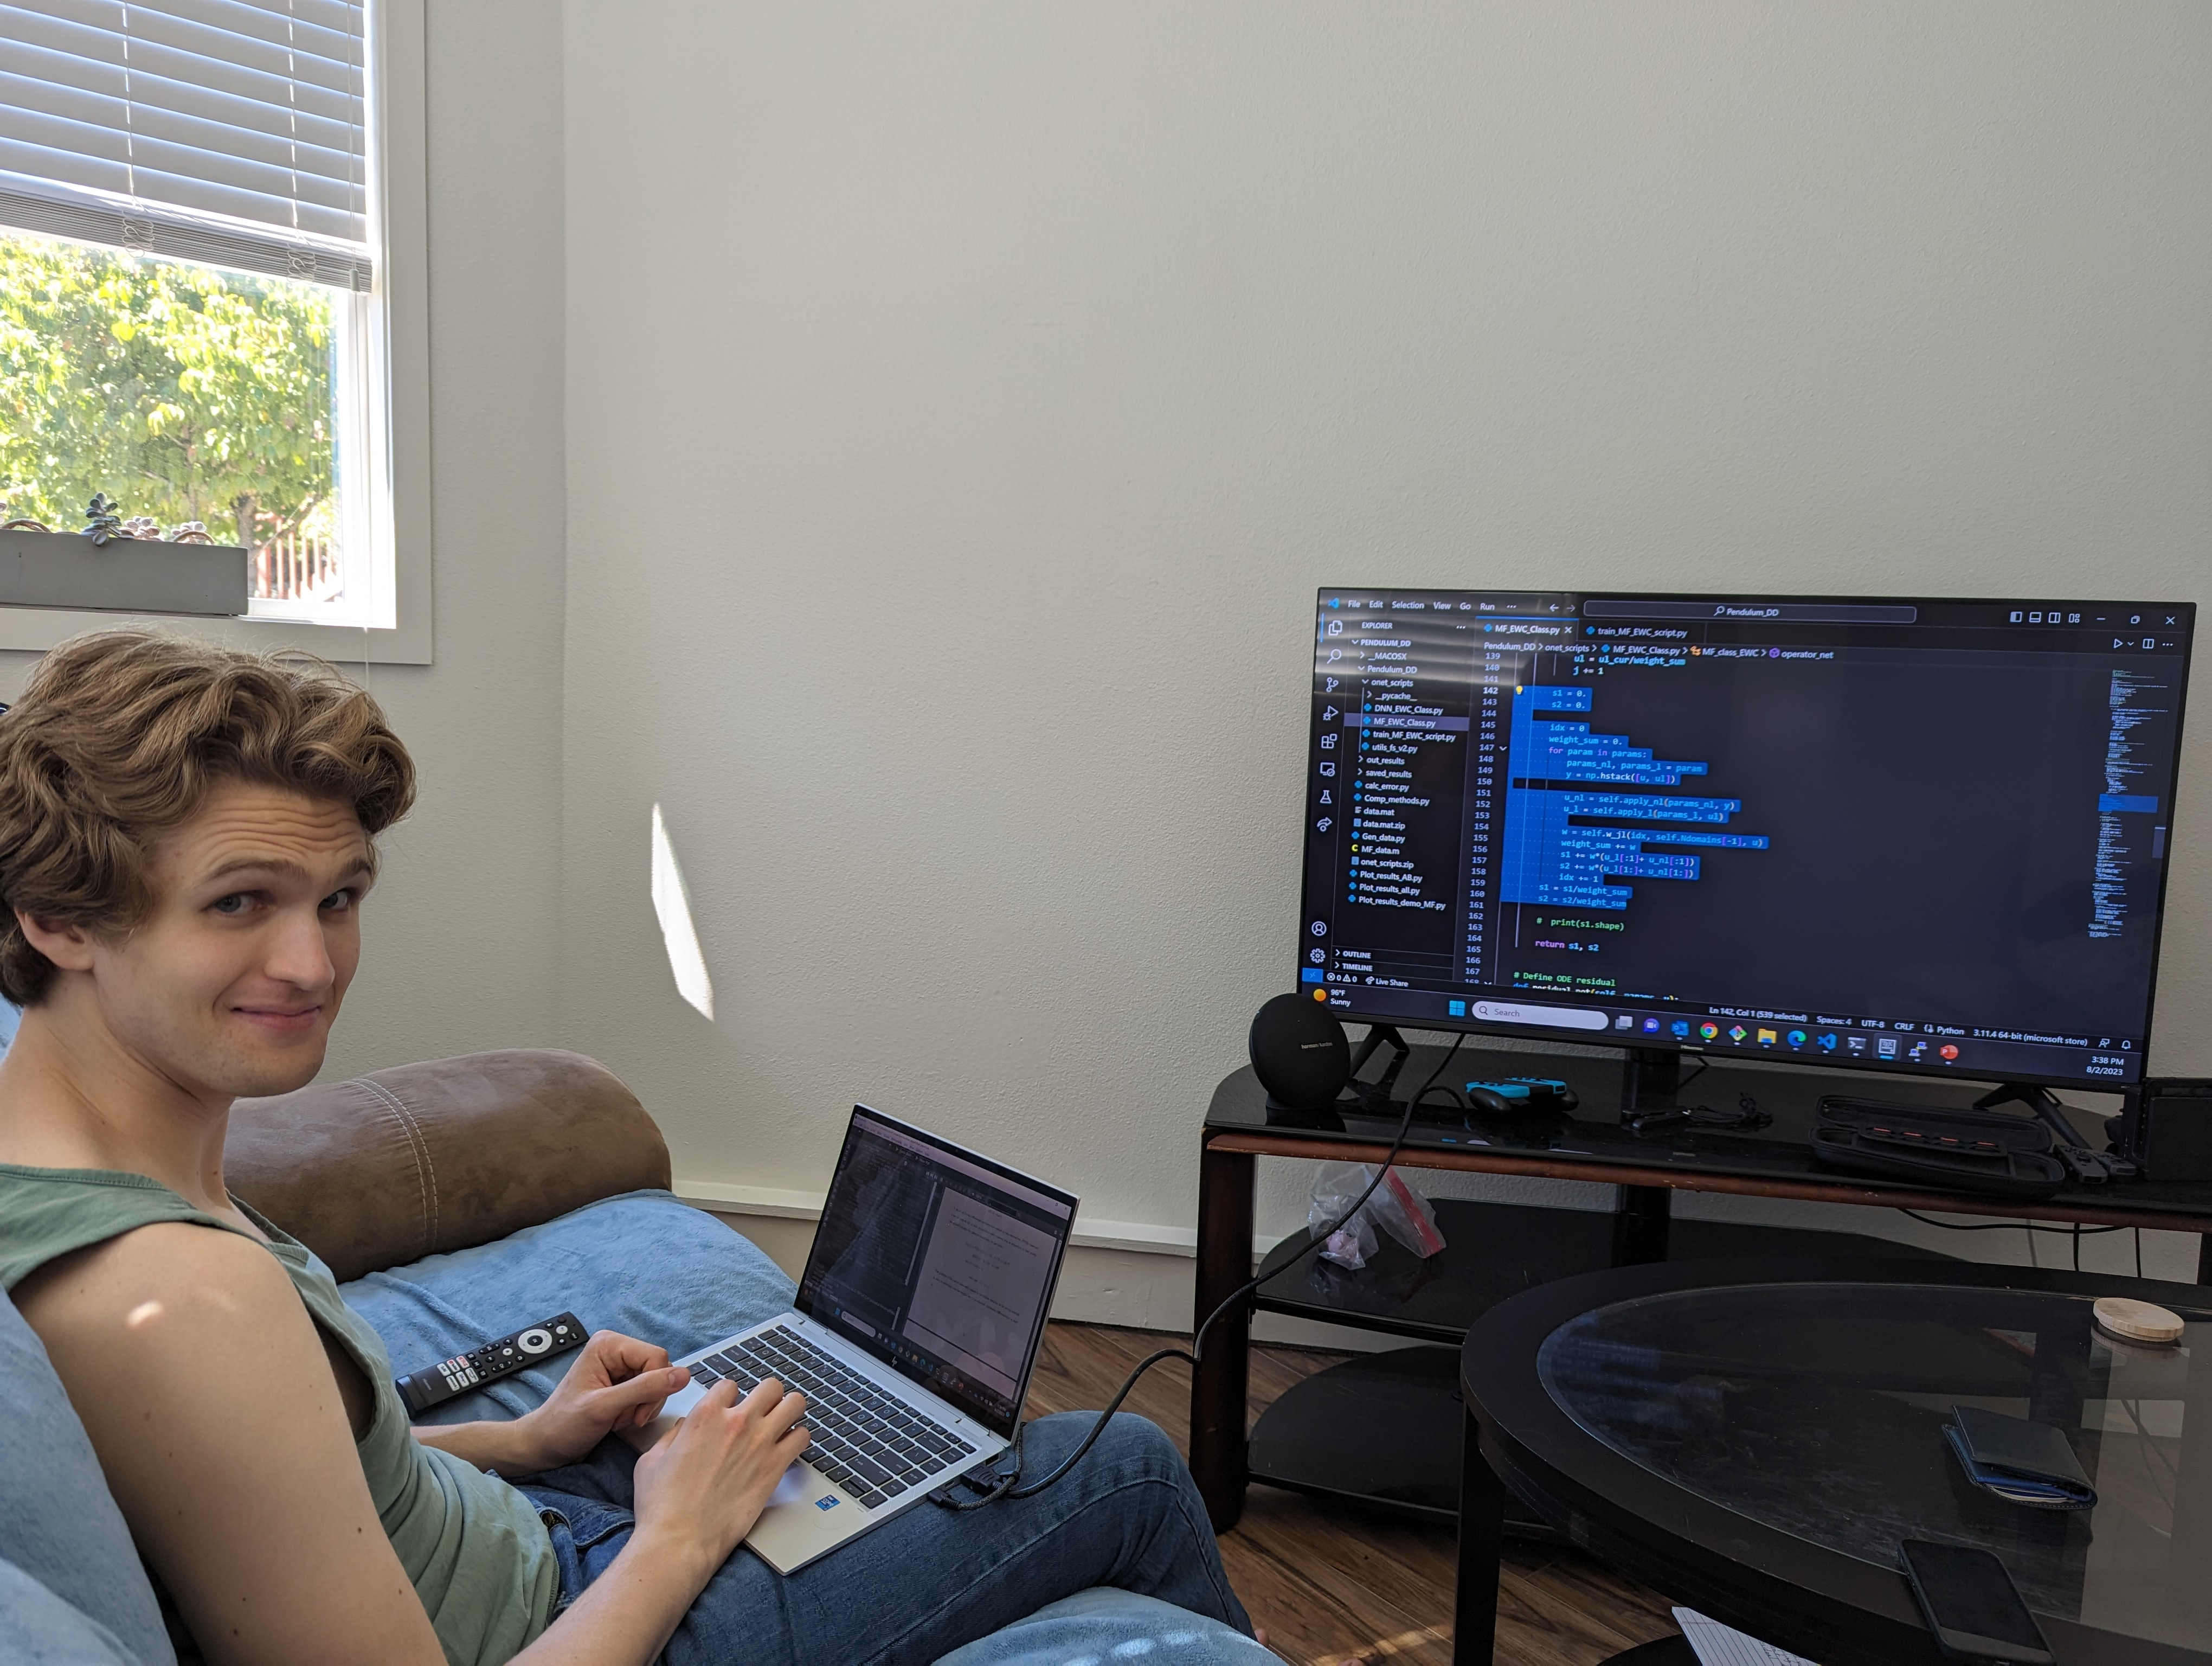
\includegraphics[width = 0.9\textwidth]{imgs/me.jpg}
\caption{My internship at Pacific Northwest National Lab was virtual. My office was anywhere I lugged my computer. On my more adventurous days I ventured all the way down to my living room to use the television as a secondary monitor. On one such day my girlfriend Caitlin Neher was kind enough to take this photo for my final report.}
\label{fig:me}
\end{figure} 

\vfill
\newpage
\section{Introduction}

Physics informed neural networks (PINNs) learn the solution to a differential equation for a given set of initial and boundary conditions \cite{pinns}. We briefly review PINNs here. Suppose that we have the following differential equation.
\begin{align} 
	u(t,x)_t + N[u(t,x)] &= 0 \quad \text{for} \quad x \in \Omega, \: t \in [0,T] \notag\\
	B[u(t,x)] &= 0 \quad \text{for} \quad x \in \partial \Omega\\
	u(0,x) &= u_0(x) \notag
\end{align} \label{eq:dq}
$N$ and $B$ are known differential operators that contain no time derivatives. PINNs construct a neural network $\~u(t,x)$ that is penalized every training step in proportion to how poorly the network satisfies the physical constraints.
\begin{align}
	\~u(t,x)_t + N[\~u(t,x)] &= l_1 \quad \text{for} \quad x \in \Omega, \: t \in [0,T] \notag \\
	B[\~u(t,x)] &= l_2 \quad \text{for} \quad x \in \partial \Omega\\
	\~u(0,x) - u_0(x)& = l_3 \notag \\
	\text{total loss}& = \lambda_1 \text{MSE}(l_1) + \lambda_2 \text{MSE}(l_2) + \lambda_3 \text{MSE}(l_3) \notag
\end{align} \label{eq:loss}
\noindent Here MSE denotes the mean squared error and $\lambda_1$, $\lambda_2$, and $\lambda_3$ determine how heavily each loss term is weighted. For some of the networks we trained in this paper we also penalize the magnitude of the weights in the hidden layers and other things. The gradient of the total loss is taken with respect to the hidden variables of the neural network to determine how the weights are to be adjusted. Automatic differentiation is used to differentiate the neural network with respect to the temporal and spatial variables. 
\par This is a simple and elegant framework. However, PINNs struggle to learn oscillatory and multi-scale solutions. They often converge to erroneous fixed point solutions in these scenarios \cite{fixedpts}. This makes sense since fixed point solutions have a small residual and small hidden weights. 
%There are a variety of methods and techniques that have been introduced to improve the convergence of PINNs. I incorporated several of these techniques into my research.
\section{Description of Project}
\par My research this summer focused on testing a new extension of PINNs: multifidelity finite basis physics informed neural networks (MFFBPINNs). This method is the combination of two other extensions of PINNs: multifidelity PINNs and multilevel finite basis PINNs.
\par Multifidelity PINNs learn from two separate data sources: a high and low fidelity data source. The multifidelity network learns the correlation between the two data sources to achieve a more accurate prediction of the true solution. This method is discussed further in Meng et al. \cite{mfpinns} and Howard et al. \cite{mfdeeponets}. This process is illustrated in Figure \ref{fig:mfpinn}.

\begin{figure}[h]
\center
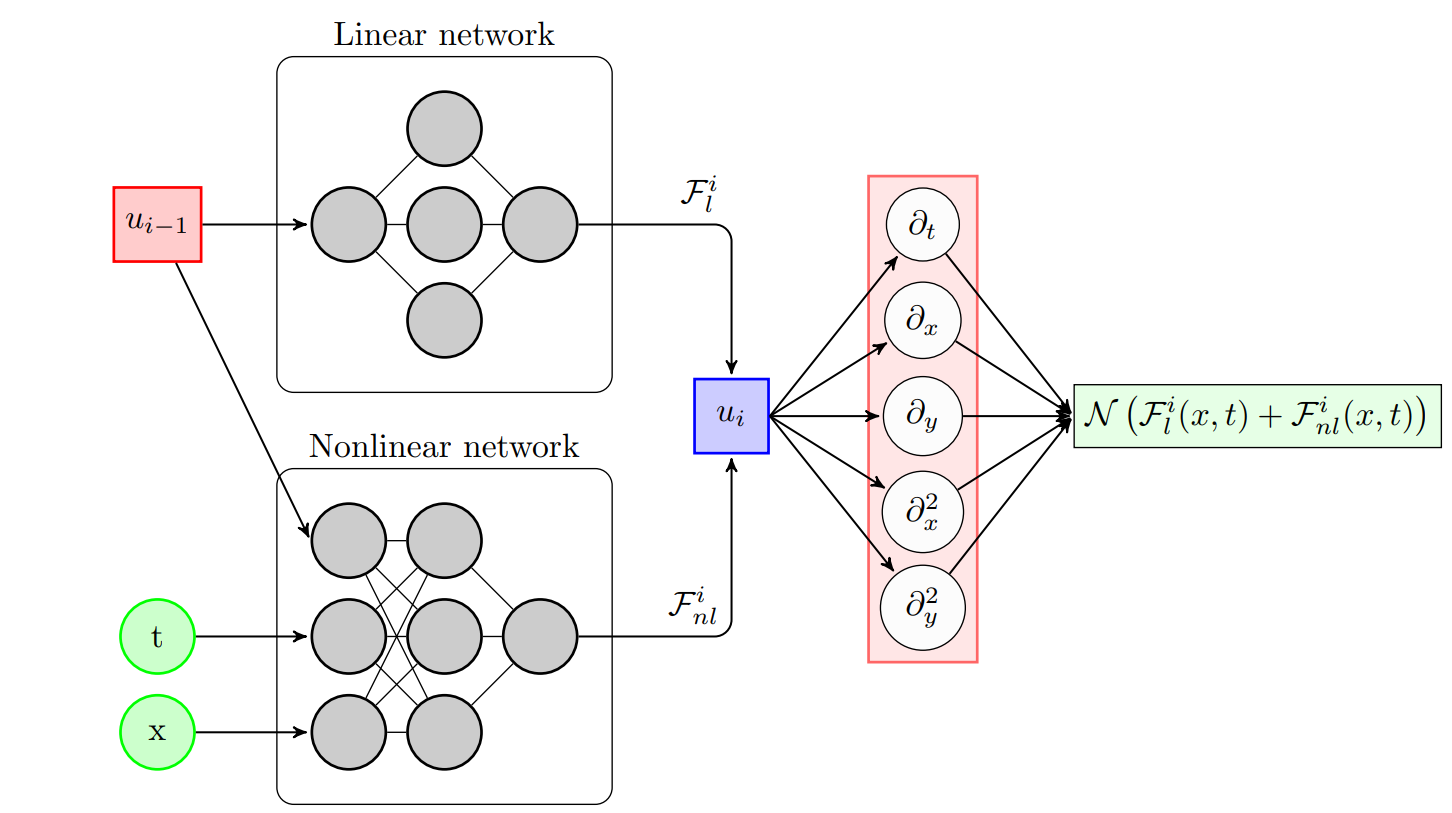
\includegraphics[width = 0.6\textwidth]{imgs/mfpinns2}
\caption{This is an illustration of a multifidelity PINN. The multifidelity PINN takes in low fidelity approximations ($u_{i-1}$) and collocation points ($x$, $t$) and outputs a new set of approximations ($u_i$) that are hopefully better than the low fidelity ones. $u_i$ is called the high fidelity prediction. This network can then be differentiated to see how well it satisfies the differential equation.}
\label{fig:mfpinn}
\end{figure} 

\par Multilevel finite basis PINNs take the problem domain and decompose it into a hierarchy of overlapping subdomains \cite{fbpinns}. A neural network is trained on each of these subdomains and the levels are averaged to get the overall solution. This process is illustrated in Figure \ref{fig:fbpinn}.\footnote{Note that Dolean et al. \cite{fbpinns} say the single fidelity solver is on level 1. In this report--everywhere other than in Figure \ref{fig:fbpinn}--we say the single fidelity solver is on level 0. Sorry for the confusion.}

\begin{figure}[t]
\center
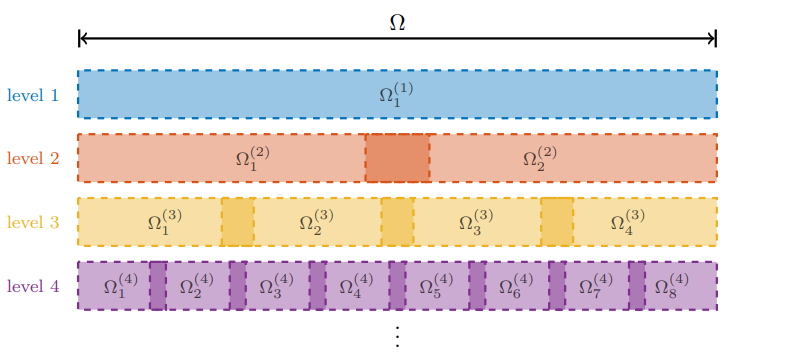
\includegraphics[width = 0.6\textwidth]{imgs/domain_decomp2}
\caption{This is a graphic illustrating multilevel finite basis PINNs from Dolean et al. \cite{fbpinns}.  Level 1 is trained first. Then, level 2 is trained to correct for the residual of level 1. Levels 1 and 2 are averaged to get the new estimate of the global solution. Level 3 is trained to correct for the errors of the new global solution. Levels 1, 2, and 3 are averaged. This process continues until a desired level of accuracy is achieved.}
\label{fig:fbpinn}
\end{figure} 

\par The subdomains in the multilevel finite basis PINN overlap to promote communication between the neural networks. We train networks together on these overlap regions to enforce that neural networks produce consistent outputs. To ensure that there is a smooth transition between the networks in these overlap regions, we define a weight function that is compactly supported on each subdomain. These weight functions are smooth and sum to one on the entire problem domain. In this study we used the same weight functions ($w_{j}^{(l)}$) as those that were used in Dolean et al. \cite{fbpinns}. We illustrate them here.

\begin{equation}
\hat{w}_j^{(l)}(t) =
    \begin{cases}
        1 & \text{if } l = 0\\
        1 + \cos(\pi(t_i - \mu_{j}^{(l)}))/\sigma_{j}^{(l)}& \text{if } l>0
    \end{cases}
\end{equation}

\begin{equation}
w_j^{(l)}(t) = \frac{\hat{w}_j^{(l)}(t)}{\sum_{j=0}^{l-1} \hat{w}_j^{(l)}(t)}
\end{equation}

\par  $l$ is the level of the MFFBPINN. Note that we start indexing at zero here as opposed to Figure \ref{fig:fbpinn} where they begin indexing at one. $j \in \{i\}_{i=0}^{2^l-1}$ is the weight function index. In the studies for this paper we studied problems with time ranging from $0$ to $T$. We set $\mu_{j}^{(l)} = \frac{Tj}{2^l-1}$ and $\sigma_{j}^{(l)} = \frac{T\delta}{2(2^l-1)}$. $\delta$ determines the amount of overlap between the subdomains. In all of our simulations $\delta = 1.9$. We can see an example of the level 2 weight functions in Figure \ref{fig:weights}.

\begin{figure}
\centering
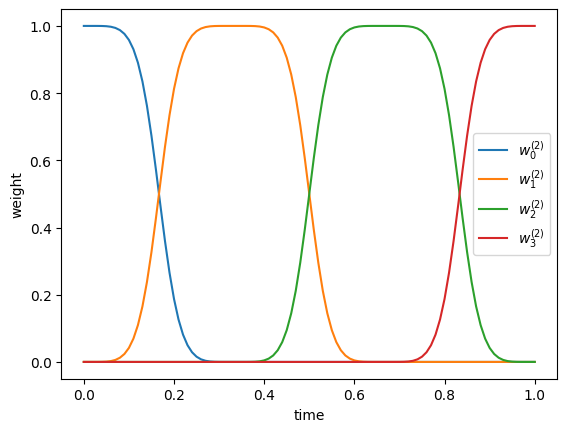
\includegraphics[width=0.45\textwidth]{imgs/weights}
\caption{The weight functions of the subdomains for the second level of the domain decomposition. In this example $T$ (the time to which the differential equation is solved) is one.}
\label{fig:weights}
\end{figure}

\par Now we can introduce MFFBPINNs. Suppose we are attempting to learn the differential equation posed in Equation \ref{eq:dq}. MFFBPINNs construct a hierarchy of neural networks. On the zeroth level of the hierarchy is a single fidelity neural network that requires no low fidelity data to make a prediction. This single fidelity method could be a classical PINN or even the solution of a numerical solver. The only caveat is that we need to be able to take spatial and temporal derivatives of this single fidelity solution. After the single fidelity network is trained on $\Omega$, the domain is broken up into a set of overlapping subdomains for the first multifidelity level: $\{\Omega^1_n\}_{n=0}^{N_1}$. Each multifidelity PINN on this level takes in the evaluation of the single fidelity PINN on the zeroth level as its low fidelity approximation to the solution. Now, the multifidelity PINNs on the first level are trained while the single fidelity network's parameters are frozen. For the second level of multifidelity PINNs the process is repeated. The domain is broken up into a new set of subdomains: $\{\Omega^2_n\}_{n=0}^{N_2}$. However, now the multifidelity networks on the first level provide the low fidelity data for the second level. This process repeats until a desired accuracy is achieved. This process is illustrated in Figure \ref{fig:mffbpinn}. 

\begin{figure}
\centering
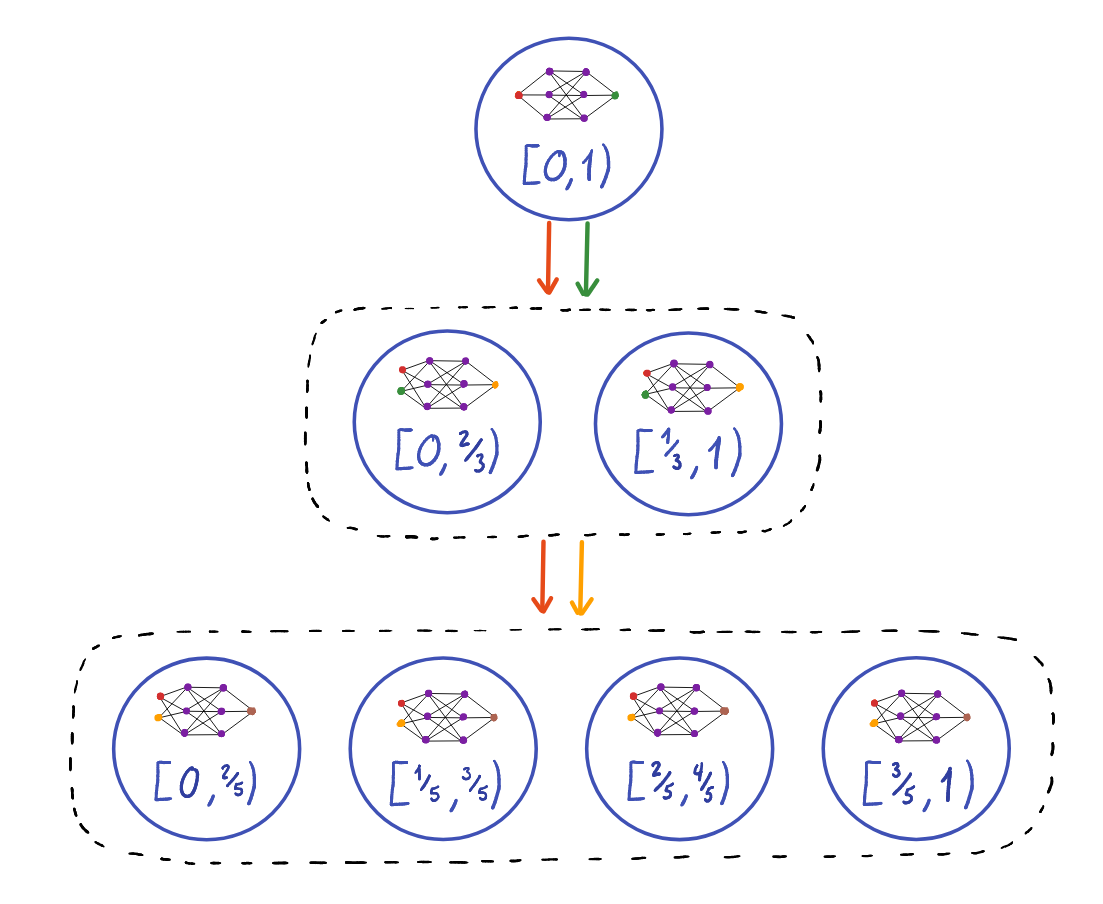
\includegraphics[width=0.5\textwidth]{imgs/mffbpinns4}
\caption{A simple diagram of the MFFBPINN algorithm for a 1D problem where the number of domains is doubled at each step. The collocation points (red) and the predictions from the previous levels are fed into the next level. Each circle is a PINN and its corresponding domain. The PINN on the zeroth level only takes in the collocation points and is therefore a single fidelity PINN. The PINNs on the subsequent levels take in the collocation points and the prediction of the previous layer, making them multifidelity PINNs.}
\label{fig:mffbpinn}
\end{figure}

\section{Contributions Made to the Project}
\subsection{Summary}
I had two tasks to accomplish during this project. The first was to create an efficient implementation of the MFFBPINN algorithm. The second was to test the MFFBPINNs on a collection of test problems. This position was ten weeks. I spent roughly the first three weeks reading up on the PINNs, setting up my work computer, learning to use the PNNL GPU cluster, and trying to understand source code that Amanda sent me. I began my attempt to improve on Amanda's source code on week four. The source code was an ad hoc implementation of the MFFBPINN algorithm set up for a damped pendulum equations. I call this code "ad hoc" because every neural network on every subdomain was evaluated on all the collocation points. However, only the points inside the domain of the PINN matter. Therefore, many points were evaluated by the network only to be zeroed out by the weight function later on. This is very inefficient. I began developing an algorithm that fixed this problem and was also very flexible so that one could generalize the implementation to higher dimensions with more complex subdomains. I spent weeks four and part of week five doing this. Towards the end of the fifth week I began trying to integrate Jax into my method. This did not work. Jax is very efficient at the cost of flexibility. I could not figure out how to integrate Jax into my algorithm. I tried for roughly a week and a half to no avail. At this point Amanda and Panos said that I should prioritize getting results over finishing the algorithm. Thus, I used the ad hoc pendulum code to produce results.  I also had to implement the domain decomposition for the wave and Allen-Cahn equations. I used this code to produce the results in this report. Creating these results took most of the time remaining in my internship.
%\begin{table}
%\resizebox{\textwidth}{!}{%
%  \begin{tabular}{cc}
%    Knuth & Lamport
%  \end{tabular}}
%\end{table}
\subsection{Results}
The results are structured as follows. The first plot for each equation shows the prediction of the true solution given by the multifidelity PINNs (or PINN) on the deepest level of the MFFBPINN. I trained two types of MFFBPINNs. (a) shows the results of a MFFBPINN where each level doubles the number of domains of the previous level. This is identical to domain decomposition (DD) process seen in Figure \ref{fig:fbpinn}. (b) shows the results of a MFFBPINN where each level only contains one PINN. There is no domain decomposition. We also show the errors of the prediction of each level of the MFFBPINNs and provide a table of the hyperparameters used during training. For each training example points were selected uniformly randomly in the domain.
\subsubsection{Pendulum Equation}
%\vspace{-5mm}
\begin{align*}
\frac{d s_1}{dt} &= s_2, & \frac{d s_2}{dt} &= \frac{s_2}{20} - g \sin{(s_1)} \\
s_1(0) &= 1 & s_2(0) &= 1
\end{align*}
%\vspace{-1cm}
\begin{figure}[htpb]
    \centering
    \begin{subfigure}{0.49\textwidth}
        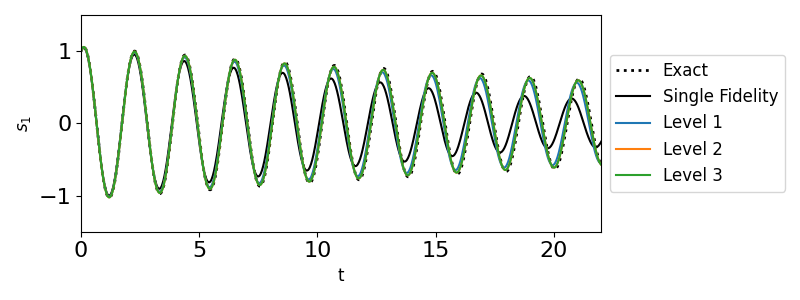
\includegraphics[width=\linewidth]{imgs/MF_loop_s1_dd}
        \caption{}
        \label{subfig:a}
    \end{subfigure}
    \hfill % Add horizontal space between subfigures and subcaptions
    \begin{subfigure}{0.49\textwidth}
        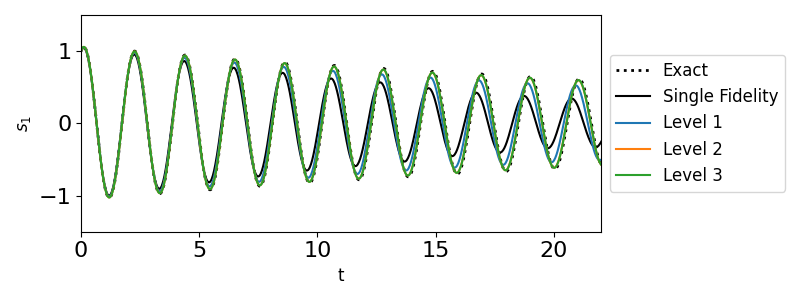
\includegraphics[width=\linewidth]{imgs/MF_loop_s1}
        \caption{}
        \label{subfig:b}
    \end{subfigure}
	\caption{Here we test two MFFBPINNs on a damped pendulum. Both methods converge to the true solution of the pendulum for up to $T=22$.}
	\label{fig:pend_res}
\end{figure}

\begin{figure}[htpb]
\centering
    \begin{subfigure}{0.4\textwidth}
	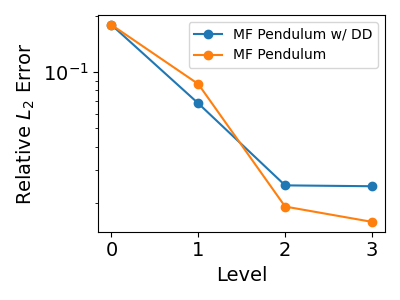
\includegraphics[width=\linewidth]{imgs/pend_errors2}
        \caption{}
        \label{subfig:a}
    \end{subfigure}
    \begin{subfigure}{0.59\textwidth}
    \scriptsize
	\begin{center}
	\begin{tabular}{|c|c|c|} 
 	\hline
	 Loss Weights & Residual				& $5$ \\  
	 			& Initial Conditions		& $1$ \\ 
	 			& Hidden Layer	& $10^-6$ \\
	\hline
	Single Fidelity	& Network Width			& $200$ \\
	Hyperparameters & Number of Hidden Layers & $5$ \\
					& Initial Learning Rate & $10^{-3}$ \\
					& Learning Rate Decay & $0.99$ \\
					& Iterations Until Decay & $2*10^3$ \\
					& Batch Size & $100$ \\
					& Iterations & $10^5$ \\
 	\hline
	Multiidelity		& Network Width			& $100$ \\
	Hyperparameters & Number of Hidden Layers & $3$ \\
					& Initial Learning Rate & $10^{-3}$ \\
					& Learning Rate Decay & $0.99$ \\
					& Iterations Between Decay & $2*10^3$ \\
					& Batch Size & $100$ \\
					& Iterations & $10^5$ \\
 	\hline
	\end{tabular}
	\end{center}
	\caption{}
     \label{subfig:b}
    \end{subfigure}
\caption{(a) The errors for the pendulum results in Figure \ref{fig:pend_res} by level. Level 0 corresponds to the single fidelity network. The performance is comparable. The addition of domain decomposition does not affect the convergence much. (b) This is the table of hyperparameters for both MFFBPINNs. All hyperparameters were the same for these tests.}
\end{figure}

\subsubsection{Wave Equation}
%\vspace{-1cm}
\begin{align*}
u_{tt} &= 4 u_{xx} \\
u(0,x) &= \sin{(\pi x)} + \frac{1}{2} \sin{(4 \pi x)} \\
u(t,1) &= 0\\ 
u(t,0) &= 0
\end{align*}
%\vspace{-1cm}
\begin{figure}[H]
    \centering
    \begin{subfigure}{0.65\textwidth}
        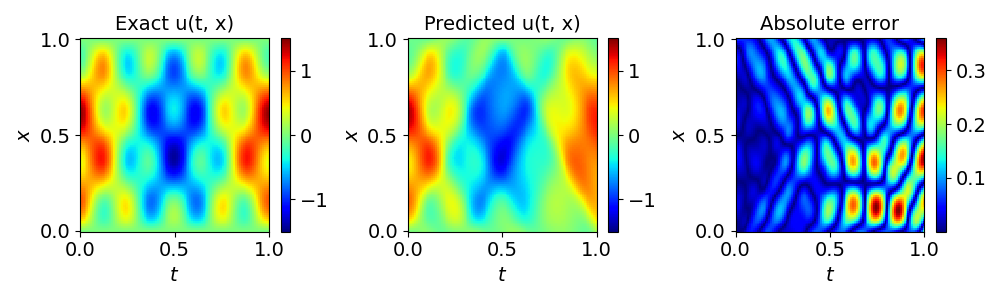
\includegraphics[width=\linewidth]{imgs/wave_dd}
        \caption{}
        \label{subfig:a}
    \end{subfigure}
    \\ % Add horizontal space between subfigures and subcaptions
    \begin{subfigure}{0.65\textwidth}
        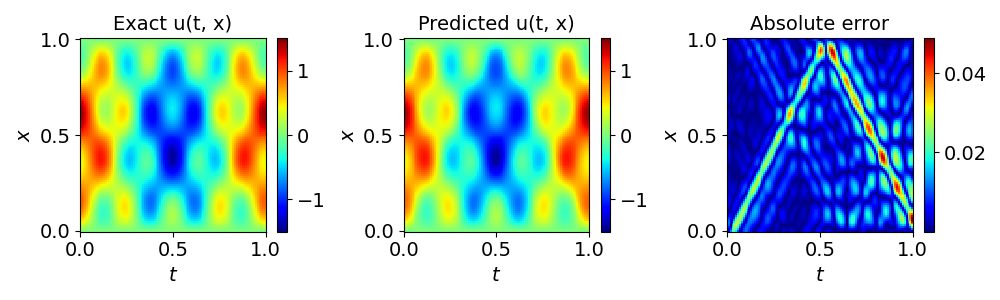
\includegraphics[width=\linewidth]{imgs/wave}
        \caption{}
        \label{subfig:b}
    \end{subfigure}
	\caption{Here we test two MFFBPINNs on the wave equation. The MFFBPINN without the domain decomposition converges here. The other does not. It seems that adding the domain decomposition can complicate convergence.}
	\label{fig:wave_res}
\end{figure}
%\vspace{-5mm}
%\begin{figure}[H]
%\centering
%    \begin{subfigure}{0.4\textwidth}
%	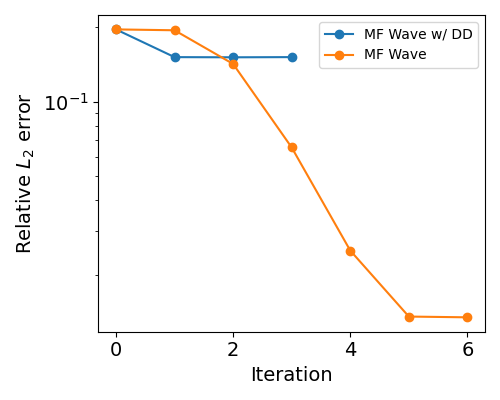
\includegraphics[width=\linewidth]{imgs/wave_errors}
%        \caption{}
%        \label{subfig:a}
%    \end{subfigure}
%    \begin{subfigure}{0.59\textwidth}
%        \scriptsize
%	\begin{center}
%	\begin{tabular}{|c|c|c|} 
% 	\hline
%	 Loss Weights & Residual				& 0 \\ 
%	        		& Boundary Conditions 	& 0 \\ 
%	 			& Initial Conditions		& 0 \\ 
%	 			& Hidden Layer	& 0 \\
%	\hline
%	Single Fidelity	& Network Width			& 0 \\
%	Hyperparameters & Number of Hidden Layers & 0 \\
%					& Initial Learning Rate & 0 \\
%					& Learning Rate Decay & 0 \\
%					& Iterations Until Decay & 0 \\
%					& Batch Size & 0 \\
%					& Iterations & $10^5$ \\
% 	\hline
%	Multifidelity	& Network Width			& 0 \\
%	Hyperparameters & Number of Hidden Layers & 0 \\
%					& Initial Learning Rate & 0 \\
%					& Learning Rate Decay & 0 \\
%					& Iterations Until Decay & 0 \\
%					& Batch Size & 0 \\
%					& Iterations & $10^5$ \\
% 	\hline
%	\end{tabular}
%	\end{center}
%	\caption{}
%     \label{subfig:b}
%    \end{subfigure}
%\caption{The errors for the wave equation results in Figure \ref{fig:wave_res} by level. The addition of domain decomposition seems to stymy the convergence. The (a) was trained for three levels and (b) was trained for 6.}
%\end{figure}

\begin{figure}[H]
\centering
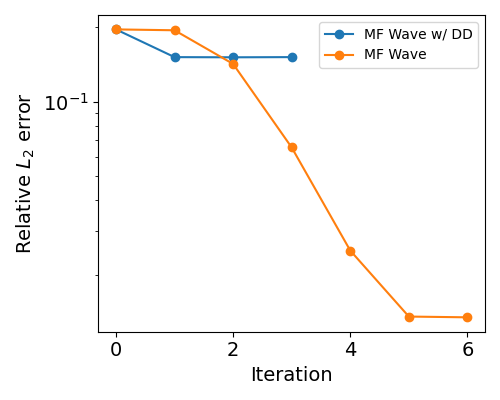
\includegraphics[width=0.45\textwidth]{imgs/wave_errors}
\caption{The errors for the wave equation results in Figure \ref{fig:wave_res} by level. The addition of domain decomposition seems to stymy the convergence. The (a) was trained for three levels and (b) was trained for 6.}
\end{figure}
\begin{figure}[H]
\centering
    \begin{subfigure}{0.49\textwidth}
        \scriptsize
	\begin{center}
	\begin{tabular}{|c|c|c|} 
 	\hline
	 Loss Weights & Residual				& 1 \\ 
	        		& Time Derivative 	& 1 \\ 
	        		& Boundary Conditions	& 20 \\
	 			& Initial Conditions		& 20 \\ 
	 			& Hidden Layer	& 0 \\
	\hline
	Single Fidelity	& Network Width			& 100 \\
	Hyperparameters & Number of Hidden Layers & 5 \\
					& Initial Learning Rate & $10^{-4}$ \\
					& Learning Rate Decay & 0.95 \\
					& Iterations Until Decay & $2*10^3$ \\
					& Batch Size & 300 \\
					& Iterations & $10^5$ \\
 	\hline
	Multifidelity	& Network Width			& 120 \\
	Hyperparameters & Number of Hidden Layers & 5 \\
					& Initial Learning Rate & $10^{-4}$ \\
					& Learning Rate Decay & 0.99 \\
					& Iterations Between Decay & $2*10^3$ \\
					& Batch Size & 300 \\
					& Iterations & $10^5$ \\
 	\hline
	\end{tabular}
	\end{center}
	\caption{}
     \label{subfig:a}
    \end{subfigure}
	\hfill
    \begin{subfigure}{0.49\textwidth}
        \scriptsize
	\begin{center}
	\begin{tabular}{|c|c|c|} 
 	\hline
	 Loss Weights & Residual				& 1 \\ 
	        		& Time Derivative 	& 1 \\ 
	        		& Boundary Conditions	& 20 \\
	 			& Initial Conditions		& 20 \\ 
	 			& Hidden Layer	& 0 \\
	\hline
	Single Fidelity	& Network Width			& 100 \\
	Hyperparameters & Number of Hidden Layers & 5 \\
					& Initial Learning Rate & $10^{-4}$ \\
					& Learning Rate Decay & 0.95 \\
					& Iterations Until Decay & $2*10^3$ \\
					& Batch Size & 300 \\
					& Iterations & $10^5$ \\
 	\hline
	Multifidelity	& Network Width			& 30 \\
	Hyperparameters & Number of Hidden Layers & 3 \\
					& Initial Learning Rate & $10^{-2}$ \\
					& Learning Rate Decay & 0.95 \\
					& Iterations Between Decay & $2*10^3$ \\
					& Batch Size & 300 \\
					& Iterations & $10^5$ \\
 	\hline
	\end{tabular}
	\end{center}
	\caption{}
     \label{subfig:b}
    \end{subfigure}
\caption{Here we have the hyperparameters for (a) the MFFBPINN without domain decomposition and (b) the MFFBPINN with domain decomposition. The derivative weight penalizes the network for not having the correct derivative at $t=0$.}
\end{figure}

\subsubsection{Allen-Cahn Equation}
%\vspace{-1cm}
\begin{align*}
u_{t} &= \frac{u_{xx}}{10,000} + 5u^3 - 5u\\
u(0,x) &= x^2 \cos{(\pi x)}\\
u(t, -1) &= u(t,1)\\
 u_x(t, -1) &= u_x(t,1)
\end{align*}
%\vspace{-1cm}
\begin{figure}[H]
    \centering
    \begin{subfigure}{0.65\textwidth}
        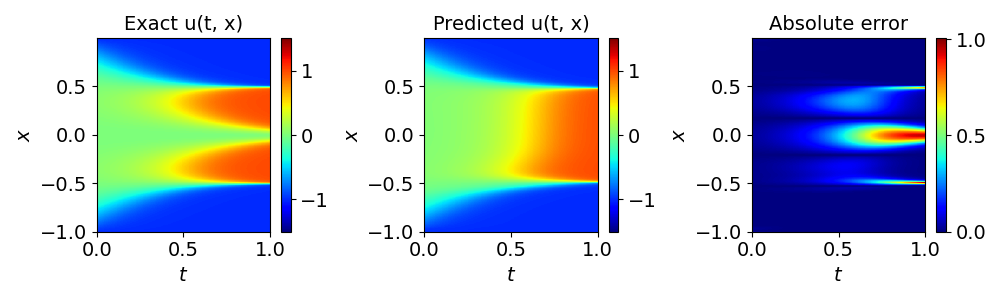
\includegraphics[width=\linewidth]{imgs/cahn_dd3}
        \caption{}
        \label{subfig:a}
    \end{subfigure}
    \\ % Add horizontal space between subfigures and subcaptions
    \begin{subfigure}{0.65\textwidth}
        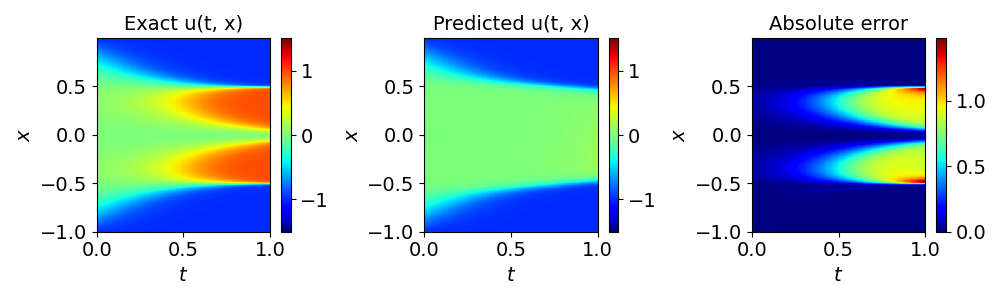
\includegraphics[width=\linewidth]{imgs/cahn3}
        \caption{}
        \label{subfig:b}
    \end{subfigure}
	\caption{Here we test two MFFBPINNs on the Allen-Cahn equation. (a) outperforms (b), however neither converge to the true solution.}
	\label{fig:cahn_res}
\end{figure}
\vspace{-5mm}

%\begin{figure}[H]
%\centering
%    \begin{subfigure}{0.4\textwidth}
%	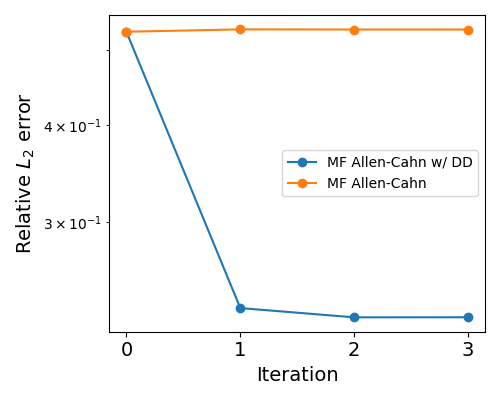
\includegraphics[width=\linewidth]{imgs/cahn_errors}
%        \caption{}
%        \label{subfig:a}
%    \end{subfigure}
%    \begin{subfigure}{0.59\textwidth}
%       \scriptsize
%	\begin{center}
%	\begin{tabular}{|c|c|c|} 
% 	\hline
%	 Loss Weights & Residual				& 0 \\ 
%	        		& Boundary Conditions 	& 0 \\ 
%	 			& Initial Conditions		& 0 \\ 
%	 			& Hidden Layer	& 0 \\
%	\hline
%	Single Fidelity	& Network Width			& 0 \\
%	Hyperparameters & Number of Hidden Layers & 0 \\
%					& Initial Learning Rate & 0 \\
%					& Learning Rate Decay & 0 \\
%					& Iterations Until Decay & 0 \\
%					& Batch Size & 0 \\
% 	\hline
%	Multifidelity	& Network Width			& 0 \\
%	Hyperparameters & Number of Hidden Layers & 0 \\
%					& Initial Learning Rate & 0 \\
%					& Learning Rate Decay & 0 \\
%					& Iterations Until Decay & 0 \\
%					& Batch Size & 0 \\
% 	\hline
%	\end{tabular}
%	\end{center}
%	\caption{}
%     \label{subfig:b}
%    \end{subfigure}
%\caption{The errors for the Allen-Cahn equation results in Figure \ref{fig:cahn_res} by level. This is the only problem we tested with heterogeneous structure. It stands to reason that the domain decomposition would help the convergence.}
%\end{figure}

\begin{figure}[H]
\centering
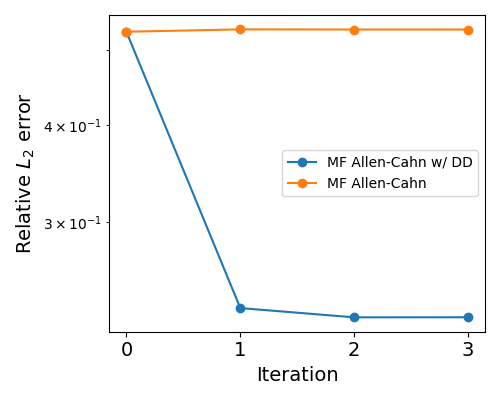
\includegraphics[width=0.45\textwidth]{imgs/cahn_errors}
\caption{The errors for the Allen-Cahn equation results in Figure \ref{fig:cahn_res} by level. This is the only problem we tested with heterogeneous structure. It stands to reason that the domain decomposition would help the convergence.}
\end{figure}

\begin{figure}[H]
\centering
    \begin{subfigure}{0.49\textwidth}
       \scriptsize
	\begin{center}
	\begin{tabular}{|c|c|c|} 
 	\hline
	 Loss Weights & Residual				& 1 \\
	        		& Time Derivative 	& 1 \\ 
	        		& Boundary Conditions 	& 1 \\ 
	 			& Initial Conditions		& 1 \\ 
	 			& Hidden Layer	& 0 \\
	\hline
	Single Fidelity	& Network Width			& 200 \\
	Hyperparameters & Number of Hidden Layers & 5 \\
					& Initial Learning Rate &  $10^{-4}$  \\
					& Learning Rate Decay & 0.99 \\
					& Iterations Until Decay & $2*10^3$ \\
					& Batch Size & 500 \\
 	\hline
	Multifidelity	& Network Width			& 30 \\
	Hyperparameters & Number of Hidden Layers & 3 \\
					& Initial Learning Rate & $10^{-3}$ \\
					& Learning Rate Decay & 0.95 \\
					& Iterations Between Decay & $2*10^3$ \\
					& Batch Size & 500 \\
 	\hline
	\end{tabular}
	\end{center}
	\caption{}
     \label{subfig:a}
    \end{subfigure}
    \begin{subfigure}{0.49\textwidth}
       \scriptsize
	\begin{center}
	\begin{tabular}{|c|c|c|} 
 	\hline
	 Loss Weights & Residual				& 1 \\
	        		& Time Derivative 	& 1 \\ 
	        		& Boundary Conditions 	& 1 \\ 
	 			& Initial Conditions		& 1 \\ 
	 			& Hidden Layer	& 0 \\
	\hline
	Single Fidelity	& Network Width			& 200 \\
	Hyperparameters & Number of Hidden Layers & 5 \\
					& Initial Learning Rate &  $10^{-4}$  \\
					& Learning Rate Decay & 0.99 \\
					& Iterations Until Decay & $2*10^3$ \\
					& Batch Size & 500 \\
 	\hline
	Multifidelity	& Network Width			& 30 \\
	Hyperparameters & Number of Hidden Layers & 3 \\
					& Initial Learning Rate & $10^{-2}$ \\
					& Learning Rate Decay & 0.95 \\
					& Iterations Between Decay & $2*10^3$ \\
					& Batch Size & 500 \\
 	\hline
	\end{tabular}
	\end{center}
	\caption{}
     \label{subfig:b}
    \end{subfigure}
\caption{Here we have the hyperparameters for (a) the MFFBPINN without domain decomposition and (b) the MFFBPINN with domain decomposition. The derivative weight penalizes the network for not having the correct derivative at $t=0$.}
\end{figure}

We see in the results that the convergence of the MFFBPINN can be sensitive to the domain decomposition. These results are the best for a range of different hyperparameters. It is important to note that these results are very preliminary and more testing needs to be done to ascertain the true effectiveness of MFFBPINNs.

\section{New Skills and Knowledge}
I gained a great deal of knowledge during the course of this internship. I began the internship by reading papers on PINNs and different methods for overcoming their convergence issues. After I had gained a sufficient basis of knowledge on PINNs I began setting up my account on the PNNL GPU cluster: Marianas. Setting up and using this account forced me to brush up my skills in a variety of tools including Anaconda, Bash, Slurm, and GitHub. After I had set up my account on the cluster I began working on implementing  MFFBPINNs to solve a variety of test problems: damped pendulum, wave equation, and Allen-Cahn equation. Working on the MFFBPINN implementation extended my knowledge of Python and introduced me to Jax. Furthermore, I did not have much hands on experience training neural networks prior to this internship. This summer has given me the opportunity to put theory into practice and see what machine learning research looks like.

\section{Experience and Impact on My Career}
Machine learning is by far the hottest research topic currently. There are many research positions in this area. Until now I was not certain what these positions would be like on a day to day basis. My internship at PNNL has given me valuable insight on this matter and will enable me to make a more informed decisions concerning my career path. Furthermore, it is likely that I do my thesis on applications of machine learning in physics. The experience from this internship will likely help me in my research.

\section{Relevance to the Mission of NSF}
The statutory mission of NSF is ``to promote the progress of science; to advance national health, prosperity, and welfare; and to secure the national defense; and for other purposes." The methods being developed in this work may one day help engineers and scientists without expertise in analytical or numerical methods solve challenging differential equations to further their research. This could in turn accelerate the development and production of technologies for the benefit of humanity.

\section{Acknowledgements}
I acknowledge and appreciate the support from the National Science Foundation Mathematical Sciences Graduate Internship program. This project was completed with support from the U.S. Department of Energy, Advanced Scientific Computing Research program, under the Scalable, Efficient and Accelerated Causal Reasoning Operators, Graphs and Spikes for Earth and Embedded Systems (SEA-CROGS) project (Project No. 80278), The computational work was performed using PNNL Institutional Computing at Pacific Northwest National Laboratory. Pacific Northwest National Laboratory (PNNL) is a multi-program national laboratory operated for the U.S. Department of Energy (DOE) by Battelle Memorial Institute under Contract No. DE-AC05-76RL01830.
\pagebreak
\bibliographystyle{plain}
\bibliography{refs}
\end{document}

%During the course of this internship, we developed two main ways to implement this algorithm. Each one is centered around how batching is done. In the first implementation, a batch containing points in the entire domain $\Omega$ is sent to the MFFBPINN. In this construction we use a tree of neural networks. The zeroth level creates its solution prediction. The networks on the first level (which are all children of the single fidelity network on the zeroth level) then look at the points in the original batch and the low fidelity solution from the zeroth layer and make their own approximation for the points that are within their subdomains. The child of each network in the second level then take in the batch points and approximations of their parents and create new approximations on the points in their subdomains and so on and so forth. A diagram illustrating this process is given in figure \ref{fig:batch1}. This method scales well with higher dimension and is rather flexible with respect to the shape of the subdomains.

%In the second implementation of the MFFBPINN, distinct batches of residual points are created for each intersection of the subdomains on the highest level. These batch points are then fed down to the neural networks on the lower levels to get the low fidelity approximations. This method is illustrated in Figure
